%!TEX encoding = UTF-8 Unicode
%!TEX TS-program = xelatex
%
% File CLARIN2018.tex
%
% Adapted for modern XeLaTeX and Unicode by desmedt@uib.no
% Otherwise contact: jwagner@computing.dcu.ie
%% 
%% Based on the style files for CLARIN2015, which were, in turn,
%% Based on the style files for CAC2014, which were, in turn,
%% Based on the style files for ACL-2014, which were, in turn,
%% Based on the style files for ACL-2013, which were, in turn,
%% Based on the style files for ACL-2012, which were, in turn,
%% based on the style files for ACL-2011, which were, in turn,
%% based on the style files for ACL-2010, which were, in turn,
%% based on the style files for ACL-IJCNLP-2009, which were, in turn,
%% based on the style files for EACL-2009 and IJCNLP-2008...

%% Based on the style files for EACL 2006 by
%%e.agirre@ehu.es or Sergi.Balari@uab.es
%% and that of ACL 08 by Joakim Nivre and Noah Smith

\documentclass[a4paper,11pt]{article}
\usepackage{CLARIN2018}
% - - - - - - - IMPORTANT - - - - - - - -
% The next three lines allow XeLaTeX, graphics import and hyperlinks, set font and language
\usepackage{xltxtra,polyglossia,graphicx,hyperref}
\setmainfont[Mapping=tex-text]{Times New Roman}
\setdefaultlanguage{english}
% If for some reason the above three lines are not compatible with your LaTeX installation,
% comment out the above three instructions and uncomment the following four instead:
%\usepackage{times}
%\usepackage{url}
%\usepackage{latexsym}
%\usepackage[english]{babel}

%\setlength\titlebox{5cm}

% You can expand the titlebox if you need extra space
% to show all the authors. Please do not make the titlebox
% smaller than 5cm (the original size); we will check this
% in the camera-ready version and ask you to change it back.

\usepackage{covington} % if needed, for linguistic examples

\begin{filecontents}{citace.bib}
@inproceedings{maekawa2000spontaneous,
  title={Spontaneous Speech Corpus of Japanese.},
  author={Maekawa, Kikuo and Koiso, Hanae and Furui, Sadaoki and Isahara, Hitoshi},
  booktitle={LREC},
  year={2000},
  organization={Citeseer}
}
@inproceedings{kruuza2012making,
  title={Making Community and ASR Join Forces in Web Environment},
  author={Kr\r{u}za, Old{\v{r}}ich and Peterek, Nino},
  booktitle={International Conference on Text, Speech and Dialogue},
  pages={415--421},
  year={2012},
  organization={Springer}
}
@article{hajek2007cesky,
  title={\v{C}esk\'{y} mystik Karel Mako\v{n}},
  author={Jurik H\'{a}jek},
  journal={Dingir},
  year={2007},
  volume={2007/4},
  pages={142--143},
  publisher={Dingir, s.r.o.},
  ISSN={1212-1371},
  editor={Zden\v{e}k Vojt\'{i}\v{s}ek}
}
\end{filecontents}

\title{Spoken Corpus of Karel Mako\v{n}}

% - - - - - - - IMPORTANT - - - - - - -
% Leave the author information empty until your paper has been accepted 

% Uncomment the following line ONLY if you need two author rows
%\setlength\titlebox{80mm} 

\author{First Author \\
  Department (optional)\\
  University of City, Country \\
  {\tt email@domain} \\\And % if needed: this makes a second column
  Second Author \\
  Department (optional)\\
  University Name without city \\
  City, Country \\
 {\tt email@domain} \\
% \AND % if needed: this makes a second row
%  Third Author \\
%  Department (optional)\\
%  University of City, Country \\
%  {\tt email@domain} \\\And
%  Fourth Author \\
%  Department (optional)\\
%  University Name without city \\
%  City, Country \\
%  {\tt email@domain} \\
}

\date{}

\begin{document}
\maketitle
\begin{abstract}
  We present a detailed view on the spoken corpus of Karel Mako\v{n}. This paper
  briefly outlines the system for processing the corpus, which has been
  published in a previous work, and elaborates on the corpus. A baseline for
  topical analysis is presented.
\end{abstract}

\section{Introduction} \label{intro}

% - - - - - - - IMPORTANT - - - - - - -
% The following footnote without marker is needed for the camera-ready
% version of the paper.
% Comment out the instructions (first text) and uncomment the 8 lines
% under "final paper" for your variant of English.
%
\blfootnote{
    %
    % for review submission
    %
    %\hspace{-0.65cm}  % space normally used by the marker
This work is licenced under a Creative Commons Attribution 4.0 International Licence.
Licence details:
\url{http://creativecommons.org/licenses/by/4.0/}
    % % final paper: en-uk version (to license, a licence)
    %
    % \hspace{-0.65cm}  % space normally used by the marker
    % This work is licensed under a Creative Commons
    % Attribution 4.0 International Licence.
    % Licence details:
    % \url{http://creativecommons.org/licenses/by/4.0/}
    %
    % % final paper: en-us version (to licence, a license)
    %
    % \hspace{-0.65cm}  % space normally used by the marker
    % This work is licenced under a Creative Commons
    % Attribution 4.0 International License.
    % License details:
    % \url{http://creativecommons.org/licenses/by/4.0/}
}

The spoken corpus of Karel Mako\v{n} is a collection of talks given in a circle
of friends in the course of late 60's or early 70's till 1991. The recordings
have been kept on magnetophone tapes until their digitization that took place
between 2010 and 2012. A complete transcription was obtained using a dedicated
ASR system and the work of the community around K.M.'s legacy. The corpus is
about 1000 hours in total length, of which about 66 have been transcribed
manually.

Most of the previous work was focused on acquiring the automatic transcription
and development of a web interface~\cite{kruuza2012making} to allow users to
access the talks and provide corrections to the existing transcription, in order
to have high-quality transcription as well as to gather more training data.

The actual content of the corpus with respect to topics, references and
statements, is on one hand quite well known
because the the domain stays
more or less consistent across the whole set. On the other hand, it is only
known vaguely and a systematic effort to analyze it is yet to be carried out.

\section{Author}

The author of the talks, Mr. Karel Mako\v{n}~\cite{hajek2007cesky} *1912
\textdagger{}1993, was giving talks in a strife to share his awareness of the
proverbial meaning of life and to give a manual to eternal life after his
release from a concentration camp during the WWII.

His steep spiritual path began in early childhood when he was subject to
repeated arm surgery without anesthesy. The pain the child suffered made him
escape mentally from inside his body, which led him to what he calls ``the
yellow light''. As a result, he felt obliged always to {\em do the right thing}.

This culminated in the age of 17, in a perceived life crissis, when he read in a
book that ``this life is the bridge to the eternal life''. The thought
captivated him and gave him a new life direction, which led to several
ecstasies.

The next culmination happened in 1939, after nine years of constant prayer for a
stronger love to God, when he was deported to the nazi concentration camp in
Sachsenhausen, as a university student. Here, he was promised certain death by a
Gestapo warden. As the nazi was approaching K.M. to kill him, he gave up his
life completely to God and the attacker unexplainably turned around in awe and
fled.

It was in that moment that Mako\v{n} obtained enlightenment, accompanied with
profound understanding of Christian symbolism. He was experiencing absolute
freedom and abundance ever since, even in the concentration camp. He also
understood the general spiritual mechanisms that conditioned his deliverance and
devoted much of his subsequent life to enabling others to learn from his
experience.

\section{Giving and Recording the Talks}

The mystical, religious and spiritual nature of Mako\v{n}'s talks put K.M. in
direct antagonism with the communist regime. The opposition was strictly
unidirectional though, as Mako\v{n} also understood the purpose of the regime
and was far from wasting his energy on a fight against it. His way of dealing
with the conflict was by staying out of wide popularity. Hence, most of the
talks have been given during regular meetings in various places of
Czechoslovakia and later the Czech Republic, in a close circle of friends.

One of the fortunate consequences of the seclusion of the talks is that there is
very little background noise on most of the recordings. Also, most of them
% TODO: kolik je od Elgra?
have been taken by a single person who used the available state-of-the-art
amateur recording technology and methods. He was also very systematic in
labeling and archiving the recordings. As a result, the majority of the base for
digitization was a set of reel-to-reel tapes labeled with ordinal indexes and a
set of cassettes labeled by year and ordinal index. The reel-to-reel tapes have
been acquired in a generous speed of 9cm/second, which granted them a very good
shield against the inevitable aging.

\section{Processing}

We don't have the resources needed to manually annotate the corpus like
e.g.~\cite{maekawa2000spontaneous}, but there are lay
volunteers willing to work on the project for the cause of tending Mako\v{n}'s
legacy.

A complete transcription is essential or at least helpful for any kind of
further processing.  Therefore,
I have focused on two major aspects of processing the material: 1. Making it
accessible to the public and 2. acquiring a complete transcription.

\subsection{Access to the Corpus}

The speech recordings are available through two sources. First and foremost,
it is in the Clarin repository, which guarantees it will be easily available no
matter what fate this project will take.

Secondly, I have created a web application for listening to the recordings
directly in the browser. The web application is also capable of displaying the
transcription synchronously. When there is an error in the transcription (which
is frequently so in case of automatically acquired ones), the user can submit a
correction.

\subsection{Complete Transcription}

Transcription of the whole corpus has been the main focus for the majority of
the time spent on the project. The concept was to transcribe a few minutes from
scratch, train a HMM-based ASR model on that, evaluate the bulk of the corpus
and feed that to the web application, as a base for the users to correct.

We only have a single speaker, a restricted domain, relatively consistent
conditions, an extensive collection of the author's original books,
translations, comments and letters to build a fitting language model. So
even very little training data should give satisfactory results and the error
rate should drop rapidly as the training data would increase.

Well, the error rate did drop as the training data increased but the accuracy of
the speech recognition was more of a challenge than I had thought. For the most
part, the users were actually using the web interface to provide a new
transcription from scratch, ignoring the way too erroneous output of the ASR,
instead of merely correcting single errors, as was meant.

Still, the community managed to provide over 66 hours of high-quality manual
transcriptions, which have been used gradually as training data. Now, the
acoustically intact recordings are automatically transcribed well enough to
allow reading along and to do full-text search.

The word error rate on our test set is currently 42\% but it is probably lower
on clean recordings and also most mistakes are in word endings, so the meaning
is comprehensible. I am currently working on a DNN acoustic
model~\cite{hannun2014deep}, so chances are the ASR score will soon rise.

\subsubsection{Acoustic Quality}

Despite of the relatively good recording technique and mostly quiet environment,
the resulting acoustic quality varies wildly. Many recordings are clearly
intelligible, while some suffer from various defects like
1. background noise in varying intensity and bandwidth,
2. altered speed,
3. clipping or faitness,
4. echo,
5. overlap of two recordings.

The varying acoustic quality is the most serious obstacle to the quality of the
automatic transcription. But it is also detrimental to the manual transcription.

To mitigate this, the web interface features since lately a user-controllable
graphical equalizer, which can help especially in the case of narrow-band noise.

\subsection{Secondary Processing Attempts}

Some limited effort was invested into further processing beyond plain
transcription. I have created a simple search engine over the transcription that
yields deep links into relevant passages in the audio. Elasticsearch was used
for this purpose, with Czech algorithmic stemmer.

Another effort was processing manually written indexes that are available for a
fraction of the recordings. These have been partly hand-written, partly typed
and are aligned using the positions of the device counter. Most of these are
scanned and some limited experiments were carried out to apply OCR. The explicit
mapping of the indexes with corresponding recordings and time-positions is yet
to be done.

\section{Topics}

In general, the whole corpus deals with a single topic that can be summarized as
a howto for entering the eternal life before the physical death. On a
finer-grained look, we can identify recurring sub-topics, like

\begin{itemize}
\item{interpretation of some passages in the New Testament, notably the parable
of the prodigal son, the parable of the talents, and the Our Father prayer,}
\item{milestone personal experiences, like the one in the concentration camp,}
\item{explaining symbolism, like the apostles as symbols for human abilities,}
\item{references to specific people, like St. Teresa of \'{A}vila or Padre Pio.}
\end{itemize}

A list of recurring topics and their identification in the sound files is a
point of future work with similarities to~\cite{skorkovska2011automatic}.
We can take the current transcription %and the few notes some listeners made
%about topics and their alignment with the audio
as a source for a baseline.
Topic is inherently a vague concept %, which I shall address when I focus on it
but for the baseline evaluation, we can take a look at some easily defined cases
like named entities. The ease about them is that we can look for their specific
word form and if it is not found, then it means the transcription is not
covering it.

Of course, there are exceptions, like saying ``the capital of Japan'' instead of
``Tokyo'' but firstly, I chose terms where this is not likely to happen and
secondly, this can only lower the recall of our baseline score, not the
precision, and we have no way of telling the recall given no annotated data
for this task.\footnote{The 50-minute test set is way too small for this kind of
task. Another source could be manual notes available to some of the recordings
but preparing them for this purpose requires some more effort.}

I have chosen the following example topics:
1. \emph{Lazarus},
2. \emph{Mithra, Mithraism},
3. \emph{Satan},
4. \emph{St. Teresa},
5. \emph{fairy-tale}.

I chose fairy-tale (Czech: \emph{poh\'{a}dka}) as a recurring topic with a
unifying word, for an example of a non-named-entity.

The search for stems of these words in the automatic part of the transcription
yielded results summed up in Table~\ref{tab:topicsearch}. For terms where there
were more than 20 hits, I have checked the first 20 but each from a different
file.

\begin{table}[htpb]
\begin{center}
\begin{tabular}{|l|l|r|r|r|}
\hline
Term & Query & hits in automatic transcription & hits in manual transcription & Precision \\
\hline
Lazarus & \texttt{lazar.*} & 16 & 14 & 8/10   \\
Mithra & \texttt{mithra.*|mitra.*} & 0 & 0 & n/a   \\
Satan & \texttt{satan.*} & 308 & 129 & 16/20   \\
St. Teresa & \texttt{terez.*} & 882 & 91 & 15/20   \\
fairy-tale & \texttt{pohádk.*} & 216 & 55 & 18/20   \\
\hline
\multicolumn{4}{|l|}{average precision} & 81.25\%\\
\hline
\end{tabular}
\caption{Text search hits in the automatically-acquired part of the
transcription}\label{tab:topicsearch}
\end{center}
\end{table}

The precision of over 80\% seems quite promising and hints that the current
quality of transcription allows for reasonable searching through the corpus.
However, the hits were all clearly audible. I met none in an acoustically defect
file, which leads to the hypothesis that those are not yet searchable to a
distantly satisfying level.

\subsubsection{Correspondence between Talks and Books}

K.M. was writing, translating and commenting books most of his life. We can
assume that the book he was just working on influenced the topic of his talks. 
For on, he translated the book \emph{El Castillo Interior}, English \emph{The
Interior Castle} by St. Teresa of Ávila in 1988. For most recordings, the year
of their acquisition is known.  Figure~\ref{fig:teresa-year} shows how many hits
for the name of the Saint are present in the transcription by recording year.

\begin{figure}[htpb]
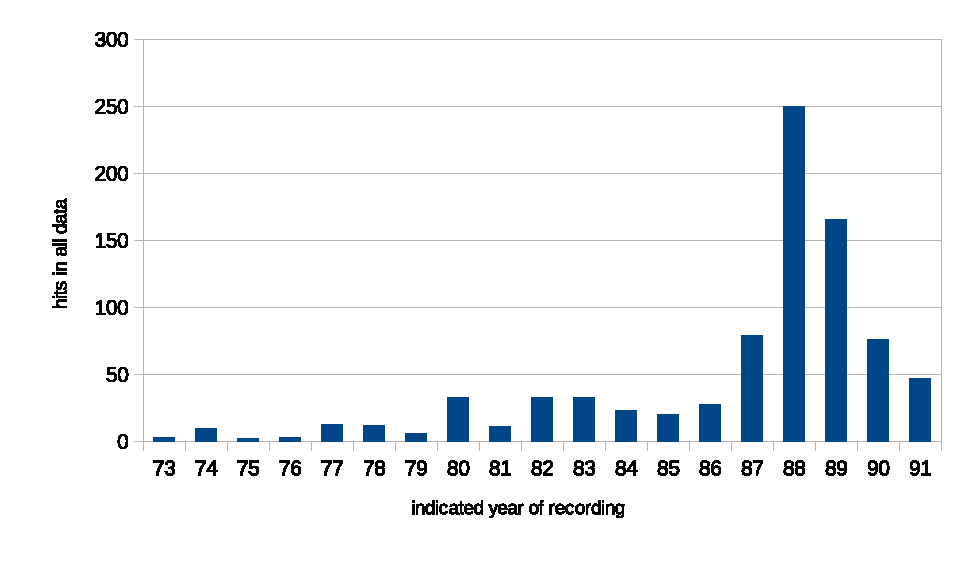
\includegraphics[scale=0.6]{rc/teresa-by-year.eps}
\caption{Number of hits for the query \texttt{terez.*} in the transcription by
alleged year of the recording}
\label{fig:teresa-year}
\end{figure}

The peak around the year 1988 supports the speculation that topics in the talks
correlate with those of books written at the same time.

\section{Conclusion}

With its length of over 1000 hours spoken by a single speaker over three
decades, the corpus of Karel Mako\v{n} is a unique piece in the Lindat/Clarin
repository. The consistent domain of Christian mystic is another of its
distinguishing features. A basis for detailed topical analysis is presented
exploiting the existing transcription and the author's books.

% 7.6\% of the corpus is annotated with 620615 : 7574994 hum : auto

%\section*{Acknowledgements}
%
%This document has been adapted from the instructions for the 
%CAC2014 proceedings, which are, in turn based on those for the
%COLING 2014 proceedings, which are, in turn, based on the ACL-2014
%proceedings compiled by Alexander Koller and Yusuke Miyao,
%which are, in turn, based on the instructions for earlier ACL proceedings,
%including those for ACL-2012 by Maggie Li and Michael
%White, those from ACL-2010 by Jing-Shing Chang and Philipp Koehn,
%those for ACL-2008 by Johanna D. Moore, Simone Teufel, James Allan,
%and Sadaoki Furui, those for ACL-2005 by Hwee Tou Ng and Kemal
%Oflazer, those for ACL-2002 by Eugene Charniak and Dekang Lin, and
%earlier ACL and EACL formats. Those versions were written by several
%people, including John Chen, Henry S. Thompson and Donald
%Walker. Additional elements were taken from the formatting
%instructions of the {\em International Joint Conference on Artificial
%  Intelligence}.


% The bibliography section below is for illustration only! Include your own bib file like this:
%\bibliography{yourbibfile}

\bibliography{citace}

\end{document}
